% \documentclass{article}
% %\usepackage[english]{babel}%
% \usepackage{graphicx}
% \usepackage{tabulary}
% \usepackage{tabularx}
% \usepackage[normalem]{ulem}
% \usepackage{cancel}
% \usepackage{tikz} 
% \usepackage{pdflscape}
% \usepackage{colortbl}
% \usepackage{lastpage}
% \usepackage{multirow}
% \usepackage{enumerate}
% \usepackage[shortlabels]{enumitem}
% \usepackage{color,soul}
% \usepackage{pdflscape}
% \usepackage{hyperref}
% %\usepackage[table]{xcolor}
% \usepackage{rotating}
% \usepackage{amsmath}
% \usepackage{fixltx2e}
% \usepackage{framed}
% \usepackage{mdframed}
% \usepackage[T1]{fontenc}
% \usepackage[utf8]{inputenc}
% \usepackage{textcomp}
% \usepackage{siunitx}
% \usepackage{ifthen}
% \usepackage{fancyhdr}
% \usepackage{gensymb}
% \usepackage{newunicodechar}
% \usepackage[document]{ragged2e}
% \usepackage[margin=1in,top=1.1in,headheight=57pt,headsep=0.1in]
% {geometry}
% \usepackage{ifthen}
% \usepackage{fancyhdr}
% \everymath{\displaystyle}
% \usepackage[document]{ragged2e}
% \usepackage{fancyhdr}
% \everymath{\displaystyle}
% \usepackage{empheq}

% \usepackage[most]{tcolorbox}

% \usepackage{booktabs} % Required for nicer horizontal rules in tables


% \usepackage{enumitem}

% %\usepackage[table,xcdraw]{xcolor}
% \usetikzlibrary{arrows}
% \linespread{2}%controls the spacing between lines. Bigger fractions means crowded lines%
% %\pagestyle{fancy}
% %\usepackage[margin=1 in, top=1in, includefoot]{geometry}
% %\everymath{\displaystyle}
% \linespread{1.3}%controls the spacing between lines. Bigger fractions means crowded lines%
% %\pagestyle{fancy}
% \pagestyle{fancy}
% \setlength{\headheight}{56.2pt}

% \definecolor{myblue}{rgb}{.8, .8, 1}
% \newcommand*\mybluebox[1]{%
% \colorbox{myblue}{\hspace{1em}#1\hspace{1em}}}

% \chead{\ifthenelse{\value{page}=1}{
\includegraphics[scale=0.3]{SCC}\\ \textbf \textbf Wastewater Constituents Analysis \& Laboratory Methods}}
% \rhead{\ifthenelse{\value{page}=1}{}{}}
% \lhead{\ifthenelse{\value{page}=1}{}{Wastewater Constituents Analysis \& Laboratory Methods}}
% \rfoot{\ifthenelse{\value{page}=1}{Module 1: WATR 048 - Spring 2019}{Module 1: WATR 048 - Spring 2019}}

% \lfoot{Shabbir Basrai}
% \cfoot{Page \thepage\ of \pageref{LastPage}}
% \renewcommand{\headrulewidth}{2pt}
% \renewcommand{\footrulewidth}{1pt}
% \begin{document}
% %\begin{empheq}[box=\mybluebox]{align}
% %a&=b\\
% %E&=mc^2 + \int_a^a x\, dx
% %\end{empheq}

% \newlist{steps}{enumerate}{1} % Defines "Steps" for enumerate as Step 1, Step 2 etc.
% \setlist[steps, 1]{label = Step \arabic*:} % Defines "Steps" for enumerate as Step 1, Step 2 etc.

% \setlist{nolistsep} % Reduce spacing between bullet points and numbered lists


%_______________________________________________________________________________________________________________________________________%
\chapterimage{Week5Ponds.jpg} % Chapter heading image

\chapter{Stabilzation Ponds}
% Chapter heading image

\begin{itemize}
\item Stabilization ponds and lagoons are bodies of water which treat wastewater using mainly natural processes including sunlight, algae and microorganisms for treating wastewater\\
\item While ponds are shallow and man-made, lagoons are bodies of water confined within natural boundaries.\\
\end{itemize}


\section{Advantages of ponds}\index{Advantages of ponds}	

\begin{itemize}	
\item Cheap to build and operate
\item Low maintenance and electrical costs
\item Do not require highly trained operational personnel
\item Provide treatment that can be equal to some secondary treatment processes and have fewer sludge handling issues.\\
\end{itemize}


\section{Disadvantages of ponds}\index{Disadvantages of ponds}	
\begin{itemize}	
\item Land intensive
\item Effluent quality varies with seasonal temperature changes
\item Suspended solids levels that can create regulatory problems.
\item System upsets almost always result in odor problems and recovery times may be weeks or months.
\item Not appropriate for colder climates
\end{itemize} 

\section{Types of Ponds}\index{Types of Ponds}	

\subsection{Anaerobic Ponds}\index{Anaerobic Ponds}	

\subsubsection{Anaerobic Ponds}\index{Anaerobic Ponds}	

\begin{itemize}	
\item Typically for treating raw sewage
\item These are deep - 10-14 feet treatment ponds which rely primarily on anaerobic bacteria to break down the organic waste.
\item Designed for BOD removal.
\item High strength wastewater may be treated.
\item Organic matter is broken down releasing releasing methane, carbon dioxide and odorous gases including hydrogen sulfide. 
\item Most of the decomposition is accomplished by acid forming bacteria. 
\item The pH in these lagoons is usually below 6.5. 
\item They are total retention and do not have an effluent discharge. 
\item The anaerobic pond must be de-sludged approximately once every 2 to 5 years
\item Organic loading of 200-1000 lbs. $BOD_5$ per acre per day
\end{itemize}

\subsection{Facultative Ponds}\index{Facultative Ponds}	

\begin{itemize}
\item The depth of facultative ponds is about 4-7 feet which is in-between the depths of anaerobic ponds (10-14 feet) and aerobic ponds 3 feet)
\item The uper layer of facultative pond is aerobic, and bottom layer is mostly anaerobic.
\item Facultative bacteria are responsible for most of the treatment that occurs in these ponds.  Facultative bacteria are bacteria which can live under both aerobic and anaerobic conditions.
\item The algae that grow in the pond are critical to the successful stabilization of the organic load. 
\item The algae will take in carbon dioxide ($CO_2$) and, through photosynthesis, use it to create sugars and release dissolved oxygen ($O_2$) that is used by the aerobic bacteria. Facultative lagoon levels should always maintain at least 4 feet of water in the pond.
\item Typically for secondary treatment - BOD removal
\item 15-50 lbs $BOD_5$ per acre per day.
\item Unused CO$_2$ will react with water to form carbonic acid - which would reduce the pH unless consumed
\item Sludge removal need is rare.  Sludge can be removed by using a raft-mounted sludge pump or by draining and dewatering the pond and removing the sludge with a front-end loader.
\end{itemize} 

				\begin{sidewaysfigure}
\begin{center}
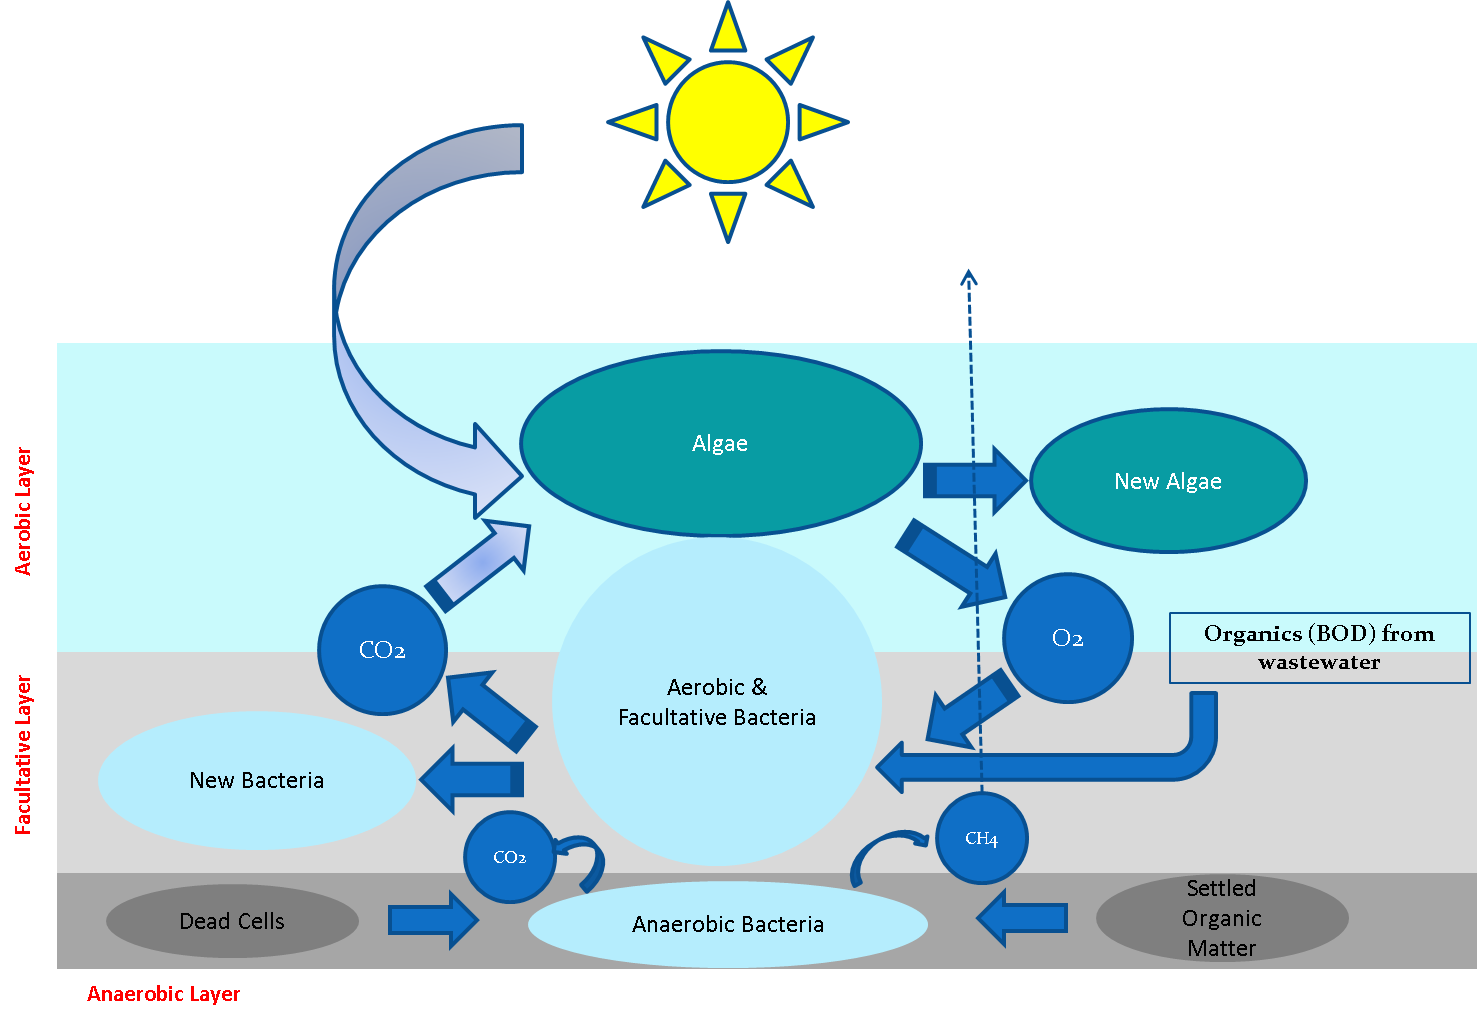
\includegraphics[scale=0.8]{StabilizationPond}\\
Facultative pond schematic
\end{center}
				\end{sidewaysfigure}
				
\subsection{Aerobic Stabilization Ponds}\index{Aerobic Stabilization Ponds}
	
Aerobic stabilization ponds are also known as: \hl{maturation}, \hl{polishing} or \hl{finishing} Pond
\begin{itemize}
\item Contain disssolved oxygen throughout entire depth of the pond.
\item Treatment is accomplished through the stabilization of organic wastes by aerobic bacteria and algae.
\item Typically for tertiary treatment
\item Designed for pathogen removal
\item Shallow - only about 3 feet deep. 
\item They are most often the final cells in a multi-staged pond system
\item They are also used as polishing ponds for tertiary treatment of trickling filter plant effluent.
\item Usually the effluent is directed into a second pond where the sludge can settle 
\item Their shallow depth allows sunlight to penetrate to the bottom of the pond to encourage algae growth and aerobic conditions throughout the pond 
\item The low solids loading found in these tertiary treatment applications means that these ponds normally have no sludge zone
\item These ponds may be mechanically aerated 
\item Aerobic polishing ponds are designed for 15-20 pounds BOD/acre/day
\item Aerobic ponds are typically designed for pathogen removal
\item Aerobic lagoon levels should always maintain at least 18 inches of water in the pond
\end{itemize}



\section{Ponds Operations and Maintenance}\index{Ponds Operations and Maintenance}

\begin{itemize}
\item Ponds and lagoons are designed as continuous discharge, controlled discharge, or no discharge.
\begin{itemize}
\item In controlled discharge ponds the wastewater is held for long periods of time before discharging. 

\item No-discharge ponds the inflow rate needs to be equal or exceed the rates of evaporation and/or percolation. 
\end{itemize}
\item Short-circuiting in a pond may be caused by poor design of inlet and outlet piping arrangements or by uncontrolled growth of water weeds.
\item Stagnant water will breed mosquitoes and can result in anaerobic conditions developing that can cause odor issues 
\item Dikes need to be maintained
\item Aquatic plants and weeds must be removed from the water. 
\item Reeds will create stagnant areas along the edge of the pond and need to be removed
\item To start a new pond, two feet of water is typically added prior to fresh starting wastewater feed. 
\item Sodium nitrate can be used to help recover from an odor-causing upset. The nitrates ($NO_3$) will provide a source of chemically bound oxygen for the bacteria to use instead of dissolved oxygen.
\item Scum control may be required
\end{itemize}

\section{Math Problems}\index{Math Problems}

\subsection{Pond Area}\index{Pond Area}

Formula: \hl{$Pond \enspace Area=Width * Length$}\\
\vspace{0.2cm}
also,     \hl{$Pond \enspace Area=\dfrac{Pond \enspace Volume}{Pond \enspace Depth}$}\\
\vspace{0.2cm}
\hl{Example Problem:}\\
A pond is 260 ft. long and 80 ft. wide. What is the area of this pond in acres?\\ 
\vspace{0.2cm}
Solution:\\
\vspace{0.2cm}
$(260*80)ft^2*\dfrac{acre}{43,560ft^2}=\boxed{0.48acre}$

\subsection{Solids Loading Rate}\index{Solids Loading Rate}


Formula: \hl{$Pond \enspace TSS \enspace loading \enspace rate =  \dfrac{lbs \enspace TSS}{day}$}  \\
\vspace{0.3cm}
\hl{Example Problem:}\\
\vspace{0.3cm}

The influent flow to a pond is 10,000 gallons/hour with a suspended solids concentration of 142mg/L in the raw wastewater.  How many lbs of suspended solids are sent to the pond daily?
\\
Solution:\\
\vspace{0.3cm}
$\dfrac{lbs \enspace TSS}{day}=10,000\dfrac{gal}{hr}*\dfrac{24hrs}{day}*\dfrac{MG}{1,000,000gal}*142\dfrac{mg}{l}*8.34=\boxed{284\dfrac{lbs \enspace TSS}{day}}$

\vspace{0.3cm}

\subsection{Organic Loading Rate}\index{Organic Loading Rate}

\vspace{0.3cm}
Formula: \hl{$Pond \enspace organic \enspace loading \enspace rate =  \dfrac{lbs \enspace BOD/day}{Area (acre)}$}  \\
\vspace{0.3cm}
\hl{Example Problem:}\\
\vspace{0.3cm}
The flow to a pond is 7.2MGD. If the pond diameter is 350 ft and the BOD in the pond influent is 170mg/L, what is the organic loading to this pond in lbs BOD/day/acre?
\\
Solution:\\
\vspace{0.3cm}
$Organic \enspace loading=\dfrac{lbs \enspace BOD \enspace per \enspace day}{area \enspace (acres)}=\dfrac{(7.2MGD \enspace * \enspace 170mg/l \enspace * \enspace 8.34)}{0.785*350^2ft^2}*\dfrac{43,560ft^2}{acre}=\boxed{\dfrac{4,624lbs \enspace BOD}{day-acre}}$

\vspace{0.3cm}

\subsection{Detention time}\index{Detention time}
\vspace{0.3cm}
Formula: \hl{$Pond \enspace detention \enspace time=\dfrac{Volume}{Flow}$}\\ 
\vspace{0.3cm}
\hl{Example Problem:}\\
A 40 acre wastewater treatment pond receives a flow of 0.6 MGD. If the pond is operated at a depth of 4ft. What is the detention time of this pond?\\
Solution:\\
$Pond \enspace detention \enspace time=\dfrac{Volume}{Flow}=\dfrac{(40*4)acre-ft}{0.6*10^6\dfrac{gal}{day}*\dfrac{ft^3}{7.48gal}*\dfrac{acre-ft}{43,560ft^3}}=\boxed{87 \enspace days}$\\
\vspace{0.3cm}


\subsection{Hydraulic Loading Rate}\index{Hydraulic Loading Rate}
Formula:\hl{$Pond \enspace hydraulic \enspace loading \enspace rate \enspace \Bigg[\dfrac{in}{day}\Bigg]=\dfrac{Flow}{Area}$}\\
also, \hl{$Pond \enspace hydraulic \enspace loading \enspace rate \Bigg[\dfrac{in}{day}\Bigg]=\dfrac{Pond \enspace depth \enspace (in)}{Pond \enspace detention  \enspace time \enspace \dfrac{Volume}{Flow}}$ }\\
The second formula above is because:\\
\vspace{0.3cm}
$Hydraulic \enspace Loading \enspace (HL)=\dfrac{Flow}{Area}$\\
\vspace{0.3cm}
$Detention \enspace time \enspace (DT)=\dfrac{Vol}{Flow} \implies Flow=\dfrac{Vol}{DT} $\\
\vspace{0.3cm}
Substituting for flow in  the HL formula above:\\
\vspace{0.3cm}
$HL=\dfrac{\dfrac{Vol}{DT}}{Area}\enspace or \enspace \dfrac{Vol}{Area*DT} \enspace \implies \boxed{HL=\dfrac{Pond \enspace Depth}{DT}} \enspace as \enspace \dfrac{Vol}{Area}=Pond \enspace Depth$\\
\vspace{0.3cm}
\textbf{Example Problems:}\\
\begin{enumerate}

\item Find hydraulic loading in inches/day for a pond given the following:
\begin{itemize}
\item Pond depth = 12ft.
\item Pond volume = 1,400,000ft3
\item Pond flow = 1,000,000gal/day
\end{itemize}
Solution:\\
$Pond \enspace hydraulic \enspace loading \enspace rate \enspace \Bigg[\dfrac{in}{day}\Bigg]=\dfrac{Flow}{Area}$\\
$ \implies\dfrac{1,000,000\dfrac{gal}{day}*\dfrac{ft^3 }{7.48gal}}{\dfrac{1,400,000ft^3}{12ft}}*12\dfrac{in}{ft}=\boxed{13.8\dfrac{in}{day}}$\\
\vspace{0.3cm}
\hl{Note:  The area of the pond was found by dividing the volume (1,000,000$ft^3$) by the pond depth (12ft)}
\vspace{0.3cm}

\item Find pond hydraulic loading in inches/day when the depth of the pond is 6 ft. and the detention time is 30 days.\\
Solution:\\



$Pond \enspace hydraulic \enspace loading \enspace rate=\dfrac{Pond \enspace depth \enspace (in)}{Pond \enspace detention  \enspace time \enspace \dfrac{Volume}{Flow}}$\\
$\implies \dfrac{6*12 \enspace inches}{30 \enspace days}=\boxed{\dfrac{2.4in}{day}}$
\end{enumerate}


